% Created by Takeuchi on Aug. 2020
\documentclass[dvipdfmx, 11pt]{beamer}

%%%% Packages %%%%%
%\usepackage{bxdpx-beamer}
%\usepackage{minijs}
%\usepackage{otf}
%\usepackage{tabularx}
%\usepackage{graphicx}
% \usepackage{graphicx}
% \usepackage{amsmath,amssymb,amsthm}
% \usepackage{multirow}
% \usepackage{url}
\usepackage{tikz}
\usetikzlibrary{arrows,shapes}
\usetikzlibrary{positioning}
% \usepackage{alltt}
% \usepackage{bm}
 \usepackage{listings,jlisting}
% \usepackage{listings}
% \lstset{
%  basicstyle=\ttfamily\scriptsize,
%  keepspaces=true,
%  escapechar=|,
%  columns=[l]{fullflexible}
% }

%%%% Fonts %%%%%
\renewcommand{\kanjifamilydefault}{\gtdefault}
% \usepackage{otf} % otfパッケージ
\usepackage[deluxe]{otf} 
\usepackage{txfonts} % 数式・英文ローマン体を Lxfont にする
% \usepackage[T1]{fontenc} % 8bit フォント
% \usepackage{minijs}
% \usepackage{textcomp} % 欧文フォントの追加
% \usepackage[utf8]{inputenc} % 文字コードをUTF-8

%%%%% Beamer %%%%%
\usetheme{Madrid}
\useinnertheme{rectangles}
%\useoutertheme{smoothbars}
\setbeamercolor{enumerate}{fg=white, bg=black}
\usefonttheme{professionalfonts}
\setbeamertemplate{frametitle}[default][center]
\setbeamertemplate{navigation symbols}{}
% \setbeamercovered{transparent} % 好みに応じてどうぞ
\setbeamertemplate{footline}[frame number]
\setbeamercolor{page number in head/foot}{fg=black} % ページ数を表示する
% \setbeamerfont{footline}{size=\normalsize,series=\bfseries}
\setbeamerfont{footline}{size=\scriptsize,series=\mdseries}
\setbeamercolor{footline}{fg=black,bg=black}
\setbeamertemplate{blocks}[rounded][shadow=true]
\setbeamertemplate{items}[ball]
% \setbeamertemplate{enumerate items}[default]
% \setbeamerfont{alerted text}{series=\bfseries}

%%%% Code %%%%%%%%%
\lstset{
 basicstyle=\ttfamily\color{black},
 keepspaces=true,
 escapechar=|,
 columns=[l]{fullflexible},
 commentstyle={\color{red}},
 stringstyle={\color{blue}},
 % literrate =%
 %   {:-}{{\textcolor{black}{:-}}}2%
 %   {,}{{\textcolor{black}{,}}}1%
 %   {.}{{\textcolor{black}{.}}}1%
}

%%%% My macro %%%%%
%%%%%%%%%%%%%%%%%%%%%%%%%%%%%%%%%%%%%%%%%%%%%%%%%%%%%%%%%%%%%%%%
% User-defined Macro
%%%%%%%%%%%%%%%%%%%%%%%%%%%%%%%%%%%%%%%%%%%%%%%%%%%%%%%%%%%%%%%%
\newcommand{\compress}{\itemsep0pt\parsep0pt\parskip0pt\partopsep0pt}
% \newcommand{\compress}{\itemsep1pt plus1pt\parsep0pt\parskip0pt}
% \newcommand{\code}[1]{\lstinline[basicstyle=\ttfamily]{#1}}
\newcommand{\gringo}{\textit{gringo}}
\newcommand{\clasp}{\textit{clasp}}
\newcommand{\clingo}{\textit{clingo}}
\newcommand{\teaspoon}{\textit{teaspoon}}
\newcommand{\sat}{\textsf{SAT}}
\newcommand{\unsat}{\textsf{UNSAT}}
% \newcommand{\web}[2]{\href{#1}{#2\ \raisebox{-0.15ex}{\beamergotobutton{Web}}}}
% \newcommand{\doi}[2]{\href{#1}{#2\ \raisebox{-0.15ex}{\beamergotobutton{DOI}}}}
% \newcommand{\weblink}[1]{\web{#1}{#1}}
% \newcommand{\imp}{\mathrel{\Rightarrow}}
% \newcommand{\Iff}{\mathrel{\Leftrightarrow}}
% \newcommand{\mybox}[1]{\fbox{\rule[.2cm]{0cm}{0cm}\mbox{${#1}$}}}
% \newcommand{\mycbox}[2]{\tikz[baseline]\node[fill=#1!10,anchor=base,rounded corners=2pt] () {#2};}
% \newcommand{\naf}[1]{\ensuremath{{\sim\!\!{#1}}}}
% \newcommand{\head}[1]{\ensuremath{\mathit{head}(#1)}}
% \newcommand{\body}[1]{\ensuremath{\mathit{body}(#1)}}
% \newcommand{\atom}[1]{\ensuremath{\mathit{atom}(#1)}}
% \newcommand{\poslits}[1]{\ensuremath{{#1}^+}}
% \newcommand{\neglits}[1]{\ensuremath{{#1}^-}}
% \newcommand{\pbody}[1]{\poslits{\body{#1}}}
% \newcommand{\nbody}[1]{\neglits{\body{#1}}}
% \newcommand{\Cn}[1]{\ensuremath{\mathit{Cn}(#1)}}
% \newcommand{\reduct}[2]{\ensuremath{#1^{#2}}}
% \newcommand{\OK}{\mbox{\textcolor{green}{\Pisymbol{pzd}{52}}}}
% \newcommand{\KO}{\mbox{\textcolor{red}{\Pisymbol{pzd}{56}}}}
% \newcommand{\code}[1]{\lstinline[basicstyle=\ttfamily]{#1}}
% \newcommand{\lw}[1]{\smash{\lower2.ex\hbox{#1}}}
\newcommand{\llw}[1]{\smash{\lower3.ex\hbox{#1}}}

\newenvironment{tableC}{%
  \scriptsize
  \renewcommand{\arraystretch}{0.9}
  \tabcolsep = 0.6mm
  % \begin{tabular}[t]{p{6mm}|rlr|rlr|rlr|rlr|rlr}\hline
  %   \multicolumn{1}{l|}{\llw{問題   }} &
  \begin{tabular}[t]{l|rlr|rlr|rlr|rlr|rlr}\hline
    \multicolumn{1}{l|}{\llw{問題}} &
    \multicolumn{3}{c|}{UD1} &
    \multicolumn{3}{c|}{UD2} &
    \multicolumn{3}{c|}{UD3} &
    \multicolumn{3}{c|}{UD4} &
    \multicolumn{3}{c}{UD5} \\
    & 
    \multicolumn{1}{c}{既知の} & & \multicolumn{1}{c|}{ASP} & 
    \multicolumn{1}{c}{既知の} & & \multicolumn{1}{c|}{ASP} & 
    \multicolumn{1}{c}{既知の} & & \multicolumn{1}{c|}{ASP} & 
    \multicolumn{1}{c}{既知の} & & \multicolumn{1}{c|}{ASP} & 
    \multicolumn{1}{c}{既知の} & & \multicolumn{1}{c}{ASP} \\
    & 
    ベスト & &  & 
    ベスト & &  & 
    ベスト & &  & 
    ベスト & &  & 
    ベスト & &  \\
    \hline
  }{%
    \hline
  \end{tabular}
}

\newcommand{\nodeVP}[3]{
  \coordinate[#2] (#1);
  \draw[fill=cyan!30] (#1)--+(-1,0)--+(0,1)--+(1,0)--cycle;
  \draw (#1)node[above]{\tiny{#3}};
  \draw[fill=black] (#1) +(-0.5,0.5)--+(0.5,0.5)--+(0,1)--cycle;
  \node[rectangle,above=0.5cm of #1,white](vp){\tiny{VP}};
  \coordinate[below=0.5cm of #1] (via_#1);
  \draw (via_#1)node[above right]{\tiny{[1..1]}};
  \draw (via_#1) +(170:0.2) arc (170:370:0.2);
  \draw (#1)--(via_#1);

}
\newcommand{\nodeTrans}[3]{
  \coordinate[#2] (#1);
  \draw[fill=cyan!30] (#1)--+(-1,0)--+(0,1)--+(1,0)--cycle;
  \draw (#1)node[above]{\tiny{#3}};
  \draw[fill=black] (#1) +(-0.5,0.5)--+(0.5,0.5)--+(0,1)--cycle;
  \node[rectangle,above=0.5cm of #1,white](vp){\tiny{VP}};
  \coordinate[below=1.7cm of #1] (via_#1);
  \draw (via_#1)node[below=0.2cm]{\tiny{[1..1]}};
  \draw (via_#1) +(135:0.2) arc (135:405:0.2);
  \draw (#1)--(via_#1);

}

\newcommand{\nodeVPdashed}[3]{
  \coordinate[#2] (#1);
  \draw[fill=cyan!30,dashed] (#1)--+(-1,0)--+(0,1)--+(1,0)--cycle;
  \draw (#1)node[above]{\tiny{#3}};
  \fill[black] (#1) +(-0.5,0.5)--+(0.5,0.5)-- +(0,1)--cycle;
  \node[rectangle,above=0.5cm of #1,white](vp){\tiny{VP}};
  \coordinate[below=0.5cm of #1] (via_#1);
  \draw (via_#1)node[above right]{\tiny{[1..1]}};
  \draw (via_#1) +(-0.2,0) arc (180:360:0.2);
  \draw (#1)--(via_#1);

}

\newcommand{\nodeV}[4]{
  \node [draw,inner xsep=2pt,#2,fill=black!10,font=\tiny] (#1){
      \begin{tabular}{l}
       #3\\
       #4\\
      \end{tabular}
  };
  \fill [black] (#1.north west)--++(0,-2mm)--++(1mm,0)--++(1mm,0)--++(0,2mm); 
  \draw (#1.north west) ++(1mm,-1mm) node[white]{\tiny{v}};
}

\newcommand{\nodeVchoiced}[4]{
  \node [draw,inner xsep=2pt,#2,fill=red!50,font=\tiny] (#1){
      \begin{tabular}{l}
       #3\\
       #4\\
      \end{tabular}
  };
  \fill [black] (#1.north west)--++(0,-2mm)--++(1mm,0)--++(1mm,0)--++(0,2mm); 
  \draw (#1.north west) ++(1mm,-1mm) node[white]{\tiny{v}};

}

%%%%%%%%%%%%%%%%%%%%%%%%%%%%%%%%%%%%%%%%%%%%%%%%%%%%
\title{車両装備仕様問題に対する\\解集合プログラミングの適用}
\author{竹内 頼人,番原 睦則,田村 直之}
\date{日本ソフトウェア科学会第37回大会(2020年度)}
\begin{document}
\begin{frame} {}
 \titlepage
\end{frame}
%%%%%%%%%%%%%%%%%%%%%%%%%%%%%%%%%%%%%%%%%%%%%%%%%%%%
\begin{frame}{車両装備仕様問題}
 \begin{itemize}
  \item 車両の装備を決定するには,販売される国や地域の法規や規制,
    地域や市場の特性,市場の嗜好や競合など十分に考慮する必要がある.
  \item 現状では専門知識をもつ技術者の多大な労力が費やされている.
  \item 車両装備仕様探索の自動化・効率化は自動車メーカーにとって重要な課題の一つである.
  % \item 日本では2020年度から,
  % 	\structure{\bf 企業別平均燃費}
  % 	(Corporate Average Fuel Efficiency; \structure{\bf CAFE})基準
  % 	と呼ばれる燃費規制が採用されている.
 \end{itemize}
 \vfill
 \begin{alertblock}{車両装備仕様問題}
  \begin{itemize}
   \item 組合せ最適化問題として定式化される.
   \item \alert{範囲制約},\alert{要求・排他制約},\alert{燃費制約},
	 \alert{初期制約}から構成される.
   \item \alert{予想販売台数を最大化}する{\bf 装備仕様}
	 (装備タイプと装備オプションの組合せ)を求めることが目的である.
  \end{itemize}
 \end{alertblock}
 \begin{itemize}
  \item 本発表では,燃費制約として企業平均燃費
	(Corporate Average Fuel Efficiency; \structure{\bf CAFE})方式を用いる.
 \end{itemize}
\end{frame}
%%%%%%%%%%%%%%%%%%%%%%%%%%%%%%%%%%%%%%%%%%%%%%%%%%%%
\begin{frame}{CAFE方式}
 \begin{itemize}
  \item 欧米で採用されており,日本でも2020年度から導入されている自動車の燃費規制
  \item 車種別ではなくメーカー全体での出荷台数を加味した平均燃費を算出し,規制をかける方式
 \end{itemize}
 \begin{exampleblock}{}
  \centering
  ここにCAFE方式の装備仕様と燃費を表すグラフ
 \end{exampleblock}
 \begin{block}{CAFE方式の特長}
  ある特定の車種では燃費基準を達成できなくても,他の車種の燃費を向上させることで
  基準を達成できることが可能な点
 \end{block}
 以降,CAFE方式に基づく車両装備仕様問題を\structure{CAFE問題}と呼ぶ.
\end{frame}
%%%%%%%%%%%%%%%%%%%%%%%%%%%%%%%%%%%%%%%%%%%%%%%%%%%%
\begin{frame}{CAFE問題の例}
 \begin{itemize}
  \item 可変性モデル(Orthogonal Variability Model; OVM)でCAFE問題の例を記述
 \end{itemize}
 \scalebox{0.8}[0.8]{%
  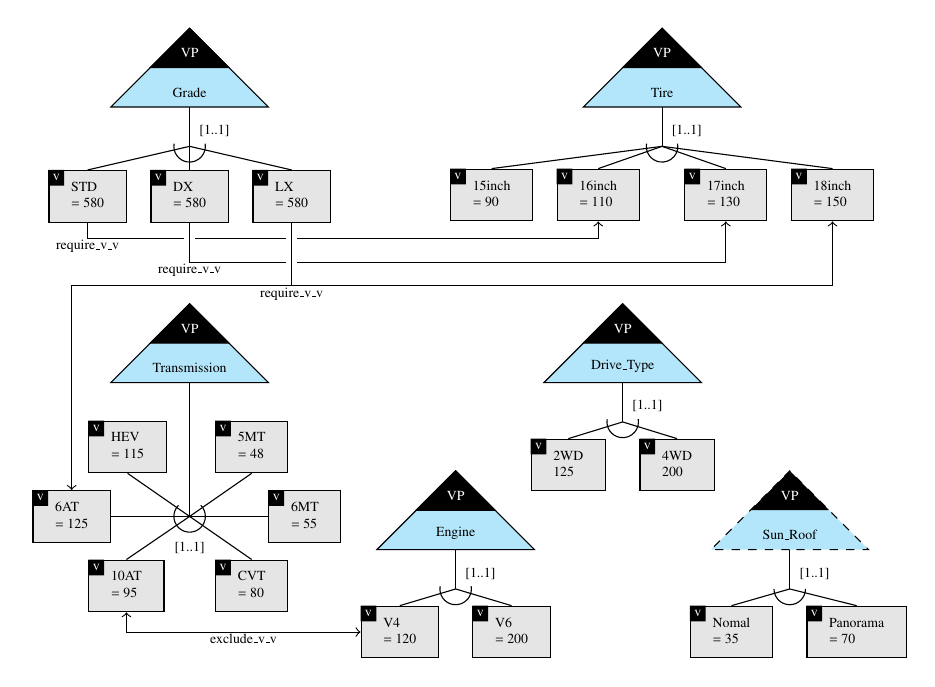
\begin{tikzpicture}
 % Grade
  \nodeVP{grade}{at={(0,0)}}{Grade};
  \nodeV{dx}{below=0.3cm of via_grade}{DX}{= 580};
  \draw(via_grade)--(dx.north);
  \nodeV{std}{left=0.3cm of dx}{STD}{= 580};
  \draw(via_grade)--(std.north);
  \nodeV{lx}{right=0.3cm of dx}{LX}{= 580};
  \draw(via_grade)--(lx.north);

  % Tire
  \nodeVP{tire}{right=6cm of grade}{Tire};
  \nodeV{16inch}{below left=0.4cm of via_tire}{16inch}{= 110};
  \nodeV{17inch}{below right=0.4cm of via_tire}{17inch}{= 130};
  \nodeV{15inch}{left=0.3cm of 16inch}{15inch}{= 90};
  \nodeV{18inch}{right=0.3cm of 17inch}{18inch}{= 150};
  \draw (via_tire)--(15inch.north);
  \draw (via_tire)--(16inch.north);
  \draw (via_tire)--(17inch.north);
  \draw (via_tire)--(18inch.north);

  % Transmission
  \nodeTrans{trans}{below=3.5cm of grade}{Transmission};
  \nodeV{6at}{left=1cm of via_trans}{6AT}{= 125};
  \nodeV{hev}{above right=0.3cm of 6at.north}{HEV}{= 115};
  \nodeV{10at}{below right=0.3cm of 6at.south}{10AT}{= 95};
  \nodeV{6mt}{right=1cm of via_trans}{6MT}{= 55};
  \nodeV{5mt}{above left=0.3cm of 6mt.north}{5MT}{= 48};
  \nodeV{cvt}{below left=0.3cm of 6mt.south}{CVT}{= 80};
  \draw (via_trans)--(10at.north);
  \draw (via_trans)--(6at.east);
  \draw (via_trans)--(hev.south);
  \draw (via_trans)--(6mt.west);
  \draw (via_trans)--(5mt.south);
  \draw (via_trans)--(cvt.north);

  % Drive_Type
  \nodeVP{drivetype}{right=5.5cm of trans}{Drive\_Type};
  \nodeV{2wd}{below left=0.3cm of via_drivetype}{2WD}{125};
  \draw (via_drivetype)--(2wd.north);
  \nodeV{4wd}{below right=0.3cm of via_drivetype}{4WD}{200};
  \draw (via_drivetype)--(4wd.north);


  % Sun_Roof
  \nodeVPdashed{sunroof}{below right=3cm of drivetype}{Sun\_Roof};
  \nodeV{nomal}{below left=0.3cm of via_sunroof}{Nomal}{= 35};
  \draw (via_sunroof)--(nomal.north);
  \nodeV{panorama}{below right=0.3cm of via_sunroof}{Panorama}{= 70};
  \draw (via_sunroof)--(panorama.north);

  % Engine
  \nodeVP{engine}{below left=3cm of drivetype}{Engine};
  \nodeV{v4}{below left=0.3cm of via_engine}{V4}{= 120};
  \draw (via_engine)--(v4.north);
  \nodeV{v6}{below right=0.3cm of via_engine}{V6}{= 200};
  \draw (via_engine)--(v6.north);
  
 

  % require
  \draw[->] (std.south)--++(0,-0.2) node[below=-1mm] {\tiny{require\_v\_v}} -|(16inch.south);
  \draw[white,line width=4pt](dx.south) ++(0,-0.1)--++(0,-0.5);
  \draw[->] (dx.south)--++(0,-0.5) node[below=-1mm] {\tiny{require\_v\_v}} -|(17inch.south);
  \draw[white,line width=4pt] (lx.south) ++(0,-0.1)--++(0,-0.8);
  \draw[->] (lx.south)--++(0,-0.8) node[below=-1mm] {\tiny{require\_v\_v}} -|(18inch.south);
  \draw[->] (lx.south)--++(0,-0.8) -|(6at.north);

  % exclude
  \draw[<->] (v4.west)-|(10at.south) node[pos=0.25,below=-1mm]{\tiny{exclude\_v\_v}};
 \end{tikzpicture}
 
 }
\end{frame}
%%%%%%%%%%%%%%%%%%%%%%%%%%%%%%%%%%%%%%%%%%%%%%%%%%%%
\begin{frame}{燃費制約と目的関数}
 \begin{itemize}
  \item FEとSVを定義
 \end{itemize}
 \begin{block}{燃費制約}
  \begin{itemize}
   \item 燃費制約にはCAFE方式
   \item 式
  \end{itemize} 
 \end{block}
 \begin{block}{目的関数}
  \begin{itemize}
   \item 販売台数最大化
  \end{itemize}
 \end{block}
\end{frame}
%%%%%%%%%%%%%%%%%%%%%%%%%%%%%%%%%%%%%%%%%%%%%%%%%%%%
\begin{frame}{CAFE問題の解}
 \begin{itemize}
  \item CAFE基準値:9.0km/L
  \item 装備仕様の数:3
  \item 初期制約:(装備仕様1, STD), (装備仕様2, DX), (装備仕様3, LX)
 \end{itemize}
 \begin{exampleblock}{}
  \centering
  \begin{tabular}{l|l|c|c|c} 
    %\multicolumn{1}{c|}{装備}   & \multicolumn{3}{c}{装備仕様} \\ \cline{2-4}
    \multicolumn{2}{l|}{装備仕様}               & 1	& 2 	 & 3	\\  \hline
    装備 & \textsf{Grade}        & \textsf{STD}    & \textsf{DX}     & \textsf{LX}\\
    &\textsf{Drive\_Type}  & \textsf{2WD}    & \textsf{2WD}    & \textsf{2WD}\\
    &\textsf{Engine}	  & \textsf{V4}     & \textsf{V6}     & \textsf{V6}\\
    &\textsf{Tire}	  & \textsf{16inch} & \textsf{17inch} & \textsf{18inch}\\
    &\textsf{Transmission} & \textsf{5MT}    & \textsf{6MT}    & \textsf{10AT}\\
    &\textsf{Sun\_Roof}    & -               & \textsf{Normal} & -  \\ \hline
    \multicolumn{2}{l|}{IWR 値の総和}           & 983  & 1,125   & 1,180 \\ %\hline
    \multicolumn{2}{l|}{燃費(km/L)}      & 10.2  & 8.9     & 8.5 \\ %\hline
    \multicolumn{2}{l|}{予想販売台数}    & 745   & 1,988   & 1,171  \\ \hline
    \multicolumn{2}{l|}{平均燃費(km/L)}  & \multicolumn{3}{c}{9.0} \\ 
    \multicolumn{2}{l|}{予想販売台数(合計)}  & \multicolumn{3}{c}{3,904} \\ 
  \end{tabular}
 \end{exampleblock}
\end{frame}
%%%%%%%%%%%%%%%%%%%%%%%%%%%%%%%%%%%%%%%%%%%%%%%%%%%%
\begin{frame}{解集合プログラミング(Answer Set Programming; ASP)}
 \begin{itemize}
 \item \structure{\bf ASP言語}は,一階論理に基づく知識表現言語の一種である.
 \item \structure{\bf ASPプログラム}は,ASPルールの有限集合である.
 \item \structure{\bf ASPシステム}は,安定モデル意味論~[Gelfond and Lifschitz '88]
   に基づく解集合を計算するシステムである.
 \item 近年,SAT技術を利用した高速なASPシステムが開発され,
%   ロボット工学,システム検証,システム生物学,
   スケジューリング,システム生物学
   など様々な分野への実用的応用が急速に拡大している.
 \end{itemize}
\vfill
 \begin{alertblock}{車両装備仕様問題に対してASPを用いる利点}
   \begin{itemize} 
    \item ASP言語の高い表現力により,各種制約を簡潔に記述できる.
    \item 高速なASPシステムを利用できる.
	  \begin{itemize}
	   \item 一階ASPプログラムを命題ASPプログラムに\alert{\bf 基礎化}した後,
		 解集合を求めるシステムが主流
	  \end{itemize}
    \item 解の最適性を保証でき,最適解の列挙も可能である.
    \item 問題を容易に拡張できる.
   \end{itemize}
 \end{alertblock}
\end{frame}
%%%%%%%%%%%%%%%%%%%%%%%%%%%%%%%%%%%%%%%%%%%%%%%%%%%%
\begin{frame}{ASPの記法}
 \begin{itemize}
  \item 論理プログラムは以下のルールの有限集合である.
 \end{itemize}
 \begin{equation}
  a_0\leftarrow a_1,\dots,a_m,\naf{a_{m+1}},\dots,\naf{a_n}
 \end{equation}
 \begin{itemize}
  \item 記号の説明.
  \item 直感的な意味は
 \end{itemize}
\end{frame}
%%%%%%%%%%%%%%%%%%%%%%%%%%%%%%%%%%%%%%%%%%%%%%%%%%%%
\begin{frame}{ASPの記法}
 \begin{itemize}
  \item ファクト
  \item 一貫性制約
 \end{itemize} 
\end{frame}
%%%%%%%%%%%%%%%%%%%%%%%%%%%%%%%%%%%%%%%%%%%%%%%%%%%%
\begin{frame}{ASPの記法}
 拡張構文
 \begin{itemize}
  \item 選択子
  \item 個数制約
  \item 重み付き個数制約
 \end{itemize}
\end{frame}
%%%%%%%%%%%%%%%%%%%%%%%%%%%%%%%%%%%%%%%%%%%%%%%%%%%%
\begin{frame}{研究目的}
 \begin{alertblock}{目的}
  ASP技術を活用して,大規模な車両装備仕様問題を効率よく解くシステム
  を実現すること.
 \end{alertblock}
 \begin{block}{既存研究}
  \begin{itemize}
   \item CAFE問題に対するASP符号化(基本符号化と呼ぶ)
   \item Babieca・神戸大学・名古屋大学 共同研究(2019)
  \end{itemize}
 \end{block}
 \begin{block}{研究内容}
  \begin{enumerate}
   \item \structure{\bf CAFE問題ソルバーを提案}
	 \begin{itemize}
	  \item \alert{\bf IWR値の和の上下限を厳密に計算する}改良符号化を考案
	        % \item この改良により,基礎化後のルール数を少なく抑えることができ,
		% 大規模な問題に対する有効性が期待できる.
	  \item オプション数を最小化する拡張符号化を考案(ソルバーの拡張性を確認)
	 \end{itemize}
   \item 企業から提供された実データを用いた実験・評価
	 \begin{itemize}
	  \item 小規模な問題に対して,最適解を得ることができた.
	  \item 大規模な問題に対して,改良符号化の有効性を確認できた.
	 \end{itemize}
  \end{enumerate}
 \end{block}
\end{frame}
%%%%%%%%%%%%%%%%%%%%%%%%%%%%%%%%%%%%%%%%%%%%%%%%%%%%
 \begin{frame}{提案するCAFE問題ソルバーの構成}
  \scalebox{0.9}{%
  \centering
    \thicklines
  \setlength{\unitlength}{1.28pt}
  \small
  \begin{picture}(280,57)(4,-10)
    \put(  0, 20){\dashbox(50,24){\shortstack{根付き全域森\\問題}}}
    \put( 60, 20){\framebox(50,24){変換器}}
    \put(120, 20){\dashbox(50,24){\shortstack{ASPファクト}}}
    \put(120,-10){\alert{\bf\dashbox(50,24){\scriptsize{\shortstack{ASP符号化\\(論理プログラム)}}}}}
    \put(180, 20){\framebox(50,24){ASPシステム}}
    \put(240, 20){\dashbox(50,24){\shortstack{根付き全域森\\問題の解}}}
    \put( 50, 32){\vector(1,0){10}}
    \put(110, 32){\vector(1,0){10}}
    \put(170, 32){\vector(1,0){10}}
    \put(230, 32){\vector(1,0){10}}
    \put(170, +2){\line(1,0){4}}
    \put(174, +2){\line(0,1){30}}
  \end{picture}  

  }
  \begin{itemize}
   \item ソルバーの
   \item 流れを
   \item 箇条書き
  \end{itemize}
  % \begin{block}{}
  %  CAFE問題ソルバーの特長を列挙
  % \end{block}
 \end{frame}
%%%%%%%%%%%%%%%%%%%%%%%%%%%%%%%%%%%%%%%%%%%%%%%%%%%%
\begin{frame}{CAFE問題のASPファクト表現}
 learning exampleのファクトを全て載せる or 一部を載せて解説をつける
\end{frame}
%%%%%%%%%%%%%%%%%%%%%%%%%%%%%%%%%%%%%%%%%%%%%%%%%%%%
\begin{frame}[fragile]{基本符号化:解候補の生成,範囲制約}
 \begin{exampleblock}{}
  \begin{lstlisting}
   (1) { vp(VP,G) } :- vp_def(VP), group(G). 
   (2) :- not vp(VP,G), require_vp(VP), group(G).
   (3) 1 { v(V,G) : v_def(V,VP,_) } 1 :- vp(VP,G).
  \end{lstlisting}
 \end{exampleblock}
 \begin{itemize}
  \item アトム\scode{vp(VP,G)}は装備仕様\scode{G}が
   	タイプ\scode{VP}を装備することを意味
  \item アトム\scode{v(V,G)}は装備仕様\scode{G}が
	オプション\scode{V}を装備することを意味
  \item (2)より,各装備仕様\scode{G}に対して,
	\scode{VP}が必須タイプならば,\scode{G}は\scode{VP}を
	装備しなければならない.
  \item (3)より,タイプ\scode{VP}を装備する装備仕様\scode{G}に対して,
	\scode{VP}のオプションからちょうど1個を実装する.
  \end{itemize}
\end{frame}
%%%%%%%%%%%%%%%%%%%%%%%%%%%%%%%%%%%%%%%%%%%%%%%%%%%%
\begin{frame}{基本符号化:要求・排他制約}
 同様にコードを説明.
\end{frame}
%%%%%%%%%%%%%%%%%%%%%%%%%%%%%%%%%%%%%%%%%%%%%%%%%%%%
\begin{frame}{基本符号化:燃費制約}
 同様にコードを説明.
\end{frame}
%%%%%%%%%%%%%%%%%%%%%%%%%%%%%%%%%%%%%%%%%%%%%%%%%%%%
\begin{frame}{基本符号化:初期制約,目的関数}
 同様にコードを説明.
\end{frame}
%%%%%%%%%%%%%%%%%%%%%%%%%%%%%%%%%%%%%%%%%%%%%%%%%%%%
\begin{frame}{基本符号化の改良点}
 \begin{block}{問題の入力}
  \begin{itemize}
   \item $VP$ 
   \item $VP*$
   \item $V$
   \item $V_i$
   \item $w_j$
  \end{itemize}
 \end{block}
 \begin{block}{IWR値の総和\code{S}の上下限}
  \[
   0 \leq \texttt{S} \leq \sum_{j\in V}w_{j}
  \]
 \end{block}
 \alert{各タイプが選択可能なオプション数の上下限,必須かどうかの別を考慮}
 \begin{alertblock}{}
  \[
   \sum_{i\in VP^{*}}\min_{j\in V_{i}}w_{j}
   \leq \texttt{S} \leq
   \sum_{i\in VP}\max_{j\in V_{i}}w_{j}
  \]
 \end{alertblock}
\end{frame}
%%%%%%%%%%%%%%%%%%%%%%%%%%%%%%%%%%%%%%%%%%%%%%%%%%%%
\begin{frame}{改良符号化}
 コードを説明.
\end{frame}
%%%%%%%%%%%%%%%%%%%%%%%%%%%%%%%%%%%%%%%%%%%%%%%%%%%%
\begin{frame}{実験}
 考案したASP符号化の有効性を評価するために実験を行なった.
 \begin{itemize}
  \item ベンチマーク問題(計15問)
	\begin{itemize}
	 \item 企業から提供された問題(3問)に対して
	 \item 5通りのCAFE基準値$X \in \{8.5, 9.0, 9.5, 10.0, 10.5km/L\}$で生成
	 \item 求める装備仕様の数$G = 3$
	\end{itemize}
	\begin{exampleblock}\small
	 \centering
	 \begin{tabular}{ l|r r r }
	  問題		& 装備タイプ数	& 装備オプション数& 要求制約数 	\\ \hline
	  small	        & 8     	& 21		& 4		\\
	  medium	& 86		& 226		& 147	\\
	  big		& 315		& 1,337		& 0		\\
	 \end{tabular}
	\end{exampleblock}
  \item ASPシステム: \textit{clingo-5.4.0}
  \item 制限時間: 1問あたり2時間
  \item 実験環境: Mac mini(3.2GHz, Intel Core i7, 64GB メモリ)
 \end{itemize}
\end{frame}
%%%%%%%%%%%%%%%%%%%%%%%%%%%%%%%%%%%%%%%%%%%%%%%%%%%%
\begin{frame}{実験結果}
 \begin{exampleblock}{}
  \centering
  \scriptsize
  \begin{tabular}{l|r|r|r}
   \lw{問題} & CAFE  & \multicolumn{2}{c}{販売台数} \\ \cline{3-4}
            & 基準値 & 基本符号化 & 改良符号化 \\\hline    
   small & 8.5   & \alert{6,021*} & \alert{6,021*}       \\
   small & 9.0   & \alert{5,007*} & \alert{5,007*}       \\
   small & 9.5   & \alert{2,688*} & \alert{2,688*}       \\
   small & 10.0  & \alert{1,318*} & \alert{1,318*}       \\
   small & 10.5  & UNSAT          & UNSAT    \\\hline
   medium & 8.5  & 6,010          & \alert{6,021}        \\
   medium & 9.0  & \alert{5,595}  & \alert{5,595}        \\
   medium & 9.5  & \alert{3,447}  & 3,430        \\
   medium & 10.0 & 2,245          & \alert{2,250}        \\
   medium & 10.5 & 1,690          & \alert{1,845}        \\\hline
   big & 8.5     & TO             & \alert{3,877}        \\
   big & 9.0     & 1,038          & \alert{4,623}        \\
   big & 9.5     & 688            & \alert{3,121}        \\
   big & 10.0    & 1,634          & \alert{2,064}        \\
   big & 10.5    & 538            & \alert{904}         \\\hline
   \multicolumn{2}{l}{最適値・最良値の数} & \multicolumn{1}{r}{6} & \alert{13} \\
  \end{tabular}
 \end{exampleblock}
 \begin{itemize}
  \item 改良符号化は,より多くの問題に対して優れた結果を示した.
  \item 大規模な問題に対する改良符号化の有効性が確認できた.
  \item 小規模な問題 small については両符号化ともに5問全てに対して最適解(あるいはUNSAT)を
	求めることができた.
 \end{itemize}	
\end{frame}
%%%%%%%%%%%%%%%%%%%%%%%%%%%%%%%%%%%%%%%%%%%%%%%%%%%%
\begin{frame}{実験結果}
 問題 small について,それぞれの符号化で最適解(あるいはUNSAT)を
 得るまでに要した CPU時間を示す.
 \begin{exampleblock}{} \centering 
  \begin{tabular}{crrr}
   問題		& CAFE基準値(km/L)  & 基本符号化(s)   & 改良符号化(s)    \\\hline
   small 	& 8.5              & 37.868         & \alert{23.318}  \\
   small	& 9.0              & 48.965         & \alert{43.362}  \\
   small	& 9.5              & \alert{95.110} & 173.172         \\
   small	& 10.0             & 99.954         & \alert{0.343}   \\
   small	& 10.5             & 439.613        & \alert{0.080}   \\\hline
   \multicolumn{2}{r}{平均}         & 144.302        & \alert{48.055}
  \end{tabular}
 \end{exampleblock}
 \begin{itemize}
  \item 5問中4問に対して,改良符号化の方が高速に解を求めた.
  \item 平均では,改良符号化のCPU時間は基本符号化の約1/3であった.
 \end{itemize}
\end{frame}
%%%%%%%%%%%%%%%%%%%%%%%%%%%%%%%%%%%%%%%%%%%%%%%%%%%%
\begin{frame}{まとめ}

\end{frame}
%%%%%%%%%%%%%%%%%%%%%%%%%%%%%%%%%%%%%%%%%%%%%%%%%%%%

\end{document}